\problemname{Track Smoothing}
Bob has the task to plan a racing track of a specific length.
He thought it is a great idea to just form a convex polygon that has exactly the required length.
Then he was told that racing cars cannot drive such sharp corners like in his plan.

He has to ensure some minimal radius for all curves in his track.
Bobs loves the shape of his track, so he don't want to change it too much.
His plan is to scale the track down around the balance point of the polygon that specifies his track.
Then, he wants to draw the new track with a line that has a constant distance to the scaled track.
The chosen distance should be minimal distance that fulfils the given minimum radius constraint.
He asks you to write a program to calculate the scale factor for a given track and minimum radius so that the resulting track has the same length as the one of his original plan.

Bob made some drawings of the first test case:

\begin{figure}[h]
\begin{minipage}[h]{.48\linewidth}
\centering
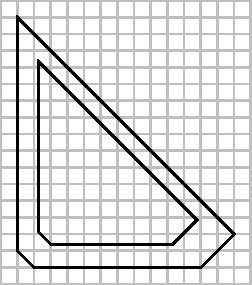
\includegraphics[scale=1.2]{scale}
\caption{Original track and scaled down track}
\end{minipage}
\begin{minipage}[h]{.48\linewidth}
\centering
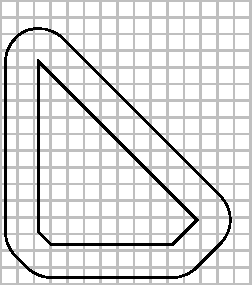
\includegraphics[scale=1.2]{dist}
\caption{Scaled down track and resulting track}
\end{minipage}
\end{figure}

\section*{Input}
The input starts with the number of test cases $t$ ($0 < t \leq 100$).
Every test case starts with a line consisting of two integers:
the minimal required radius $r$ and the number of points $n$ of the original track polygon ($0 \leq r \leq 1\,000$; $3 \le n \le 10\,000$).
Then $n$ lines follow, where each line specifies 2D-coordinates as two integers $x_i$ and $y_i$ ($-10\,000 \le x_i, y_i \le 10\,000$). $(0,0)$ is the lower left corner.
These are the coordinates of the original track in counterclockwise direction.
You may safely assume that the area of the given polygon is non-empty.

\section*{Output}
For each test case print out one line.
If it is possible to construct a course according to the above description, output the scaling factor, ``{\tt Not possible}'' otherwise.
The factor must have a relative or absolute error smaller than $10^{-5}$.
